\documentclass[sigconf,nonacm]{acmart}

\usepackage{graphicx}
\usepackage{booktabs}
\usepackage{amsmath}
\usepackage{multirow}
\usepackage{hyperref}

\begin{document}

\title{Paraphraser Fingerprinting: Can We Identify the Rewriter from the Text Alone?}

\author{CS6120 Project Report}
\affiliation{%
  \institution{Northeastern University}
  \city{Seattle}
  \state{WA}
  \country{USA}
}

\begin{abstract}
Different language models leave distinct stylistic traces---``fingerprints''---when paraphrasing text.
We investigate whether these fingerprints are detectable through two complementary evaluation paradigms: (1)~a \emph{duplicate detection} task where a Detective identifies which two of five paraphrased outputs share the same origin, and (2)~a harder \emph{pairwise classification} task where the Detective must match all four paraphrasers across two independently paraphrased texts.
Using human translations from the PAR3 corpus alongside LLM paraphrasers, we find that duplicate detection achieves 55--67\% accuracy across three Detective models (baseline 10\%), while pairwise classification achieves 22\% perfect-match accuracy (baseline 4.2\%).
Notably, human paraphrases from PAR3 are the \emph{easiest} to identify (62\% individual match rate), while Sonnet~4.6 proves hardest (34\%).
These results confirm that paraphraser fingerprinting is feasible and that both human and machine rewriters produce distinguishable patterns.
\end{abstract}

\maketitle

% ============================================================
\section{Problem Description}
% ============================================================

Large language models (LLMs) are increasingly used to paraphrase, rewrite, and polish text.
A natural question arises: \emph{do different models leave distinct traces when they paraphrase?}
If so, it may be possible to identify \emph{which} model produced a given rewrite---analogous to identifying the ``wood grain'' of an AI model.

This question has practical implications for AI-generated text detection, academic integrity, intellectual property, and understanding model behavior.
Prior work on AI text detection has focused on distinguishing human-written from machine-generated text~\cite{mitchell2023detectgpt}, but the finer-grained problem of \emph{paraphraser attribution}---identifying which specific model performed a rewrite---remains underexplored.

We address this through two task formulations:
\begin{enumerate}
    \item \textbf{Duplicate Detection.} Given 5 paraphrased outputs from 4 paraphrasers (one contributing two outputs), identify the duplicate pair.
    \item \textbf{Pairwise Classification.} Given two source texts each paraphrased by the same 4 systems, match each Group~A output to its corresponding Group~B output produced by the same system.
\end{enumerate}

% ============================================================
\section{Dataset}
% ============================================================

Unlike our earlier work which relied entirely on dynamically generated source texts, we now incorporate the \textbf{PAR3 corpus}~\cite{par3}---a dataset of paragraph-level human translations of literary works.
Each PAR3 entry contains multiple independent English translations of the same foreign-language paragraph, which serve as natural human paraphrases.

This design provides two key advantages:
\begin{enumerate}
    \item \textbf{Pre-existing human paraphrases.} PAR3 provides 2--5 independent human translations per paragraph, enabling a ``human paraphraser'' without requiring live annotation. We use one translation as the source text and the others as the human paraphraser's outputs.
    \item \textbf{Diverse literary text.} PAR3 spans multiple languages and literary styles (Dostoevsky, Voltaire, Verne, etc.), providing natural variation in source text complexity.
\end{enumerate}

We filter PAR3 for groups with $\geq 3$ translations (to support the duplicate case where the human paraphraser must produce two outputs) and minimum 100 characters per translation, yielding 100--150 candidate groups per run.

For each trial, the source text selection is \emph{random} from the pool (no Auditor LLM selection), ensuring unbiased coverage.

% ============================================================
\section{Experimentation and Results}
% ============================================================

\subsection{Experimental Setup}

\paragraph{Framework Architecture.}
Our system consists of three roles:
\begin{itemize}
    \item \textbf{Auditor}: Selects source texts from the PAR3 pool.
    \item \textbf{Detective} (LLM): Analyzes paraphrased outputs and identifies fingerprints. Tested with three models: Claude Sonnet~4.6, GPT-4.1, and Gemini~2.5~Pro.
    \item \textbf{Paraphrasers}: Two configurations tested:
    \begin{itemize}
        \item \emph{Weak}: Human (PAR3), Llama-3.1-8B, Gemini-2.5-Flash, DIPPER
        \item \emph{Strong}: Human (PAR3), Claude Sonnet~4.6, Gemini~2.5~Pro, GPT-5.4
    \end{itemize}
\end{itemize}

All LLM requests are parallelized (8 concurrent calls per trial) and results are saved incrementally to support resumption from interruptions.

\paragraph{Baselines.}
\begin{itemize}
    \item Duplicate detection: $\frac{1}{\binom{5}{2}} = 10\%$ (choose 2 of 5).
    \item Pairwise classification: $\frac{1}{4!} = 4.17\%$ (1 correct permutation of 4).
\end{itemize}

% -------------------------------------------------------
\subsection{Experiment 1: Duplicate Detection}
% -------------------------------------------------------

Each trial presents 5 shuffled paraphrases (one paraphraser duplicated) and asks the Detective to identify the pair.
Runs use 10 trials each (1 warmup), with 5--10 independent runs per configuration.

\paragraph{Detective Model Comparison.}

\begin{figure}[t]
    \centering
    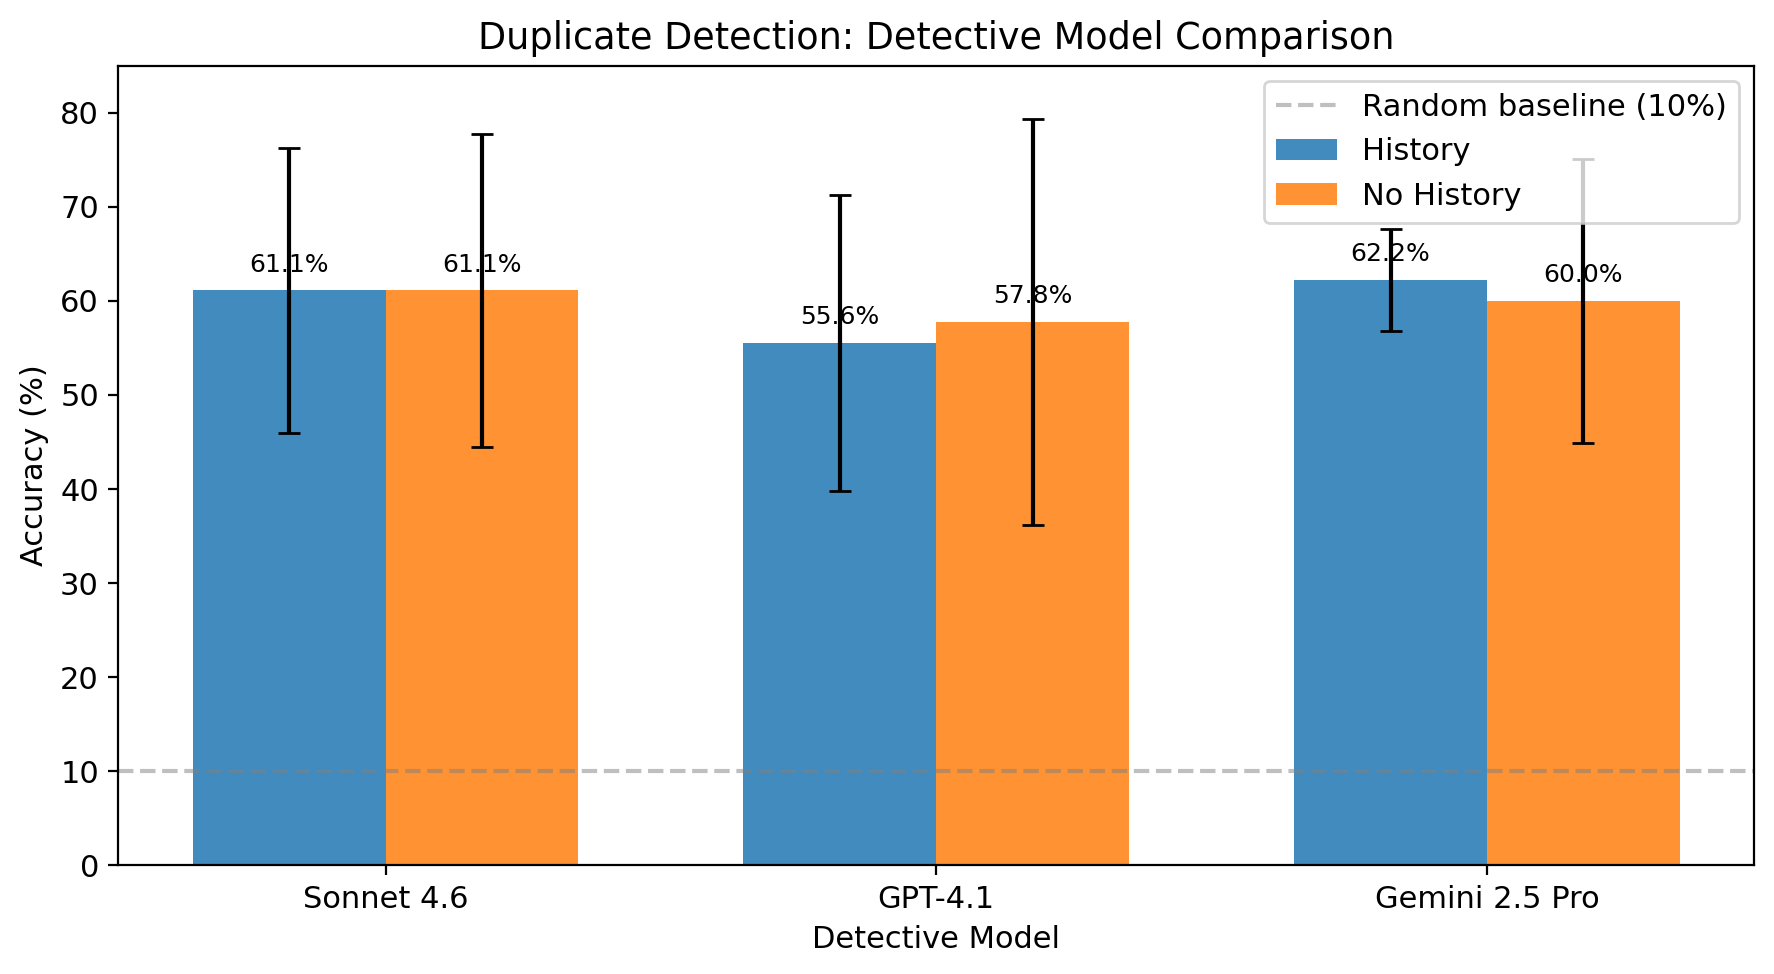
\includegraphics[width=\linewidth]{figures/fig3_detective_comparison.png}
    \Description{Grouped bar chart comparing three detective models across history and no-history conditions, all around 55-62\%.}
    \caption{Duplicate detection accuracy across three Detective models, with and without access to past trial history. All models perform significantly above the 10\% baseline, but no model or history condition is clearly superior.}
    \label{fig:detective_cmp}
\end{figure}

\begin{table}[t]
\caption{Duplicate detection accuracy by Detective model and history condition (weak paraphrasers).}
\label{tab:detective}
\centering
\begin{tabular}{llccc}
\toprule
\textbf{Detective} & \textbf{History} & \textbf{Runs} & \textbf{Mean} & \textbf{SD} \\
\midrule
Sonnet 4.6     & Yes & 10 & 61.1\% & 15.1\% \\
Sonnet 4.6     & No  & 10 & 61.1\% & 16.7\% \\
GPT-4.1        & Yes &  5 & 55.6\% & 15.7\% \\
GPT-4.1        & No  &  5 & 57.8\% & 21.5\% \\
Gemini 2.5 Pro & Yes &  5 & 62.2\% &  5.4\% \\
Gemini 2.5 Pro & No  &  5 & 60.0\% & 15.1\% \\
\bottomrule
\end{tabular}
\end{table}

Three findings emerge from Table~\ref{tab:detective} and Figure~\ref{fig:detective_cmp}:
\begin{enumerate}
    \item All detectives achieve 55--62\% accuracy, well above the 10\% baseline.
    \item \textbf{History provides no benefit}: the with-history and no-history conditions produce nearly identical results for all three models (Sonnet: 61.1\% vs.\ 61.1\%; GPT-4.1: 55.6\% vs.\ 57.8\%; Gemini: 62.2\% vs.\ 60.0\%).
    \item Gemini~2.5~Pro has the lowest variance (SD=5.4\% with history), suggesting more consistent reasoning.
\end{enumerate}

\paragraph{Weak vs.\ Strong Paraphrasers.}

\begin{figure}[t]
    \centering
    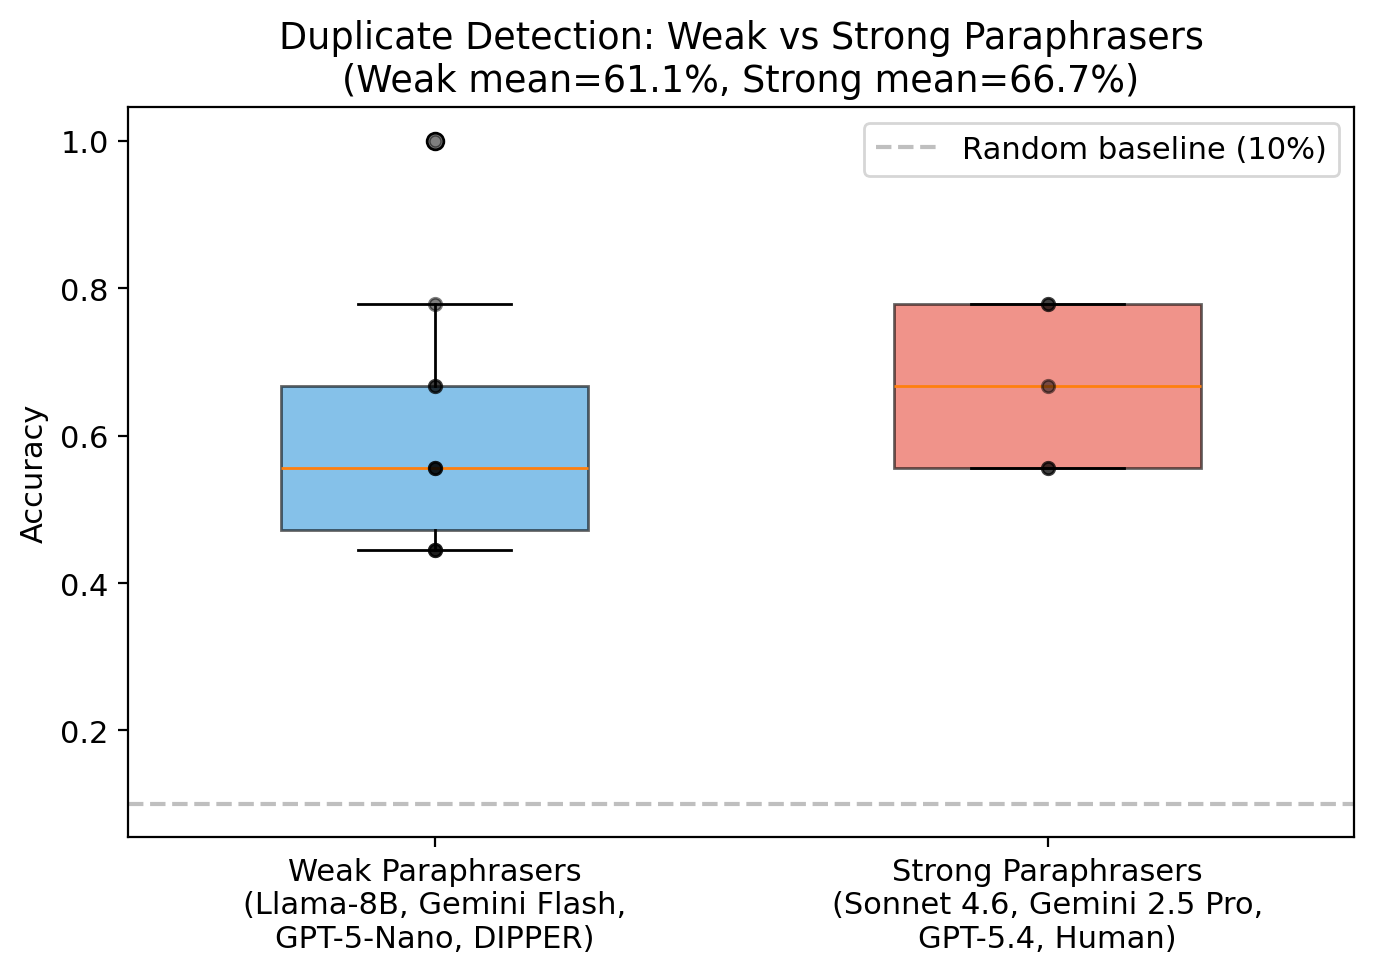
\includegraphics[width=0.85\linewidth]{figures/fig4_weak_vs_strong.png}
    \Description{Box plot comparing weak (mean 61.1\%) and strong (mean 66.7\%) paraphraser detection accuracy.}
    \caption{Duplicate detection accuracy for weak vs.\ strong paraphraser sets. Strong models are \emph{more} detectable (66.7\% vs.\ 61.1\%), suggesting that capable models develop more distinctive rewriting styles.}
    \label{fig:weak_vs_strong}
\end{figure}

Counter-intuitively, stronger paraphrasers are \emph{easier} to detect (Figure~\ref{fig:weak_vs_strong}).
The strong set (Sonnet~4.6, Gemini~2.5~Pro, GPT-5.4) yields 66.7\% detection accuracy vs.\ 61.1\% for the weak set (Llama-8B, Gemini Flash, DIPPER).
This suggests that more capable models develop more consistent and distinctive ``voices'' when paraphrasing, creating stronger fingerprints.

% -------------------------------------------------------
\subsection{Experiment 2: Pairwise Classification}
\label{sec:classification}
% -------------------------------------------------------

The pairwise classification task is substantially harder than duplicate detection.
Two source texts are drawn from PAR3, and all four paraphrasers independently rewrite both texts.
The Detective receives two groups of four shuffled outputs and must produce a complete matching---identifying which Group~A output corresponds to which Group~B output (same paraphraser).
A trial is scored correct only if \textbf{all four matches are correct}.

We ran 50 non-repeating trials with the strong paraphraser set (Human, Sonnet~4.6, Gemini~2.5~Pro, GPT-5.4), Sonnet~4.6 as Detective, no history.

\paragraph{Overall Accuracy.}

\begin{figure}[t]
    \centering
    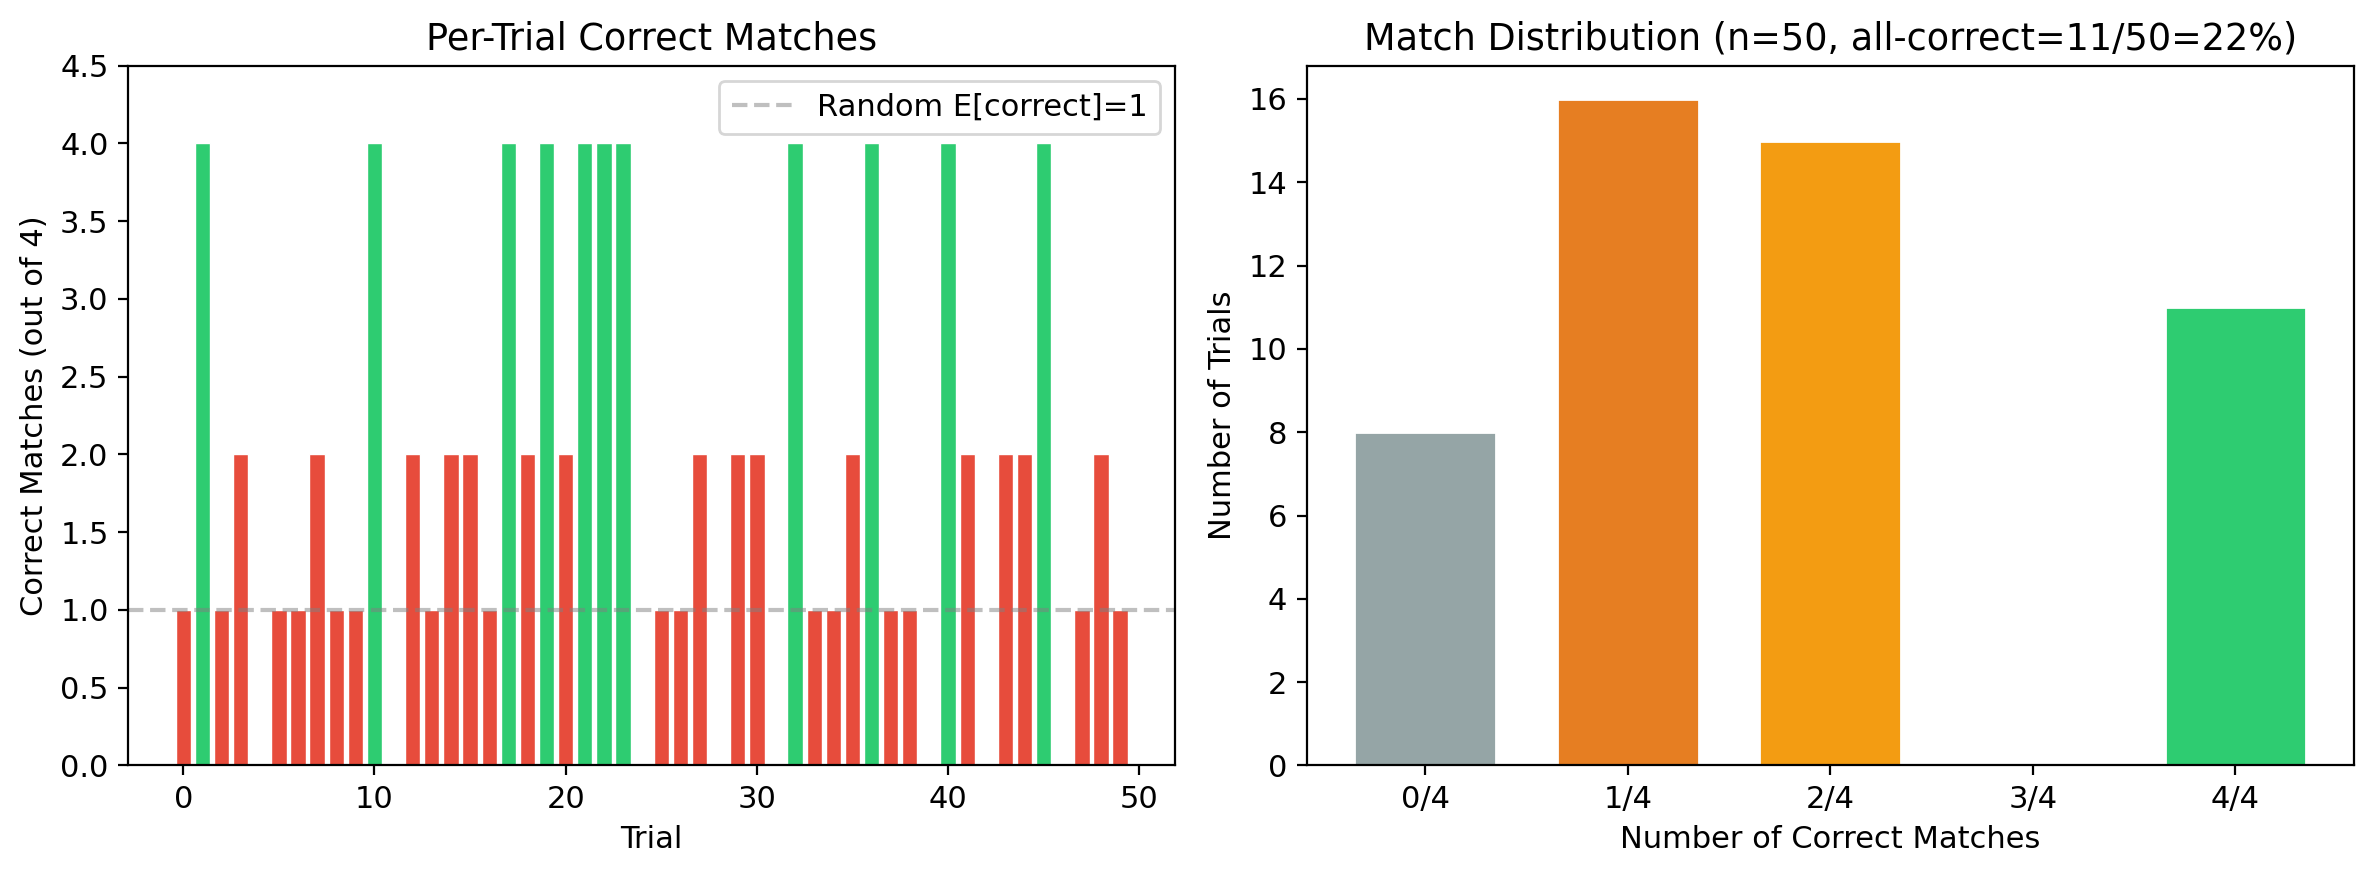
\includegraphics[width=\linewidth]{figures/fig1_classification_main.png}
    \Description{Left: per-trial bar chart of correct matches (0--4), with green bars for 4/4. Right: distribution showing 11/50 trials with all 4 correct.}
    \caption{Pairwise classification results over 50 trials. Left: per-trial correct matches (green = all 4 correct). Right: distribution of match counts. The Detective achieves 22\% perfect-match accuracy (11/50), far above the 4.17\% random baseline.}
    \label{fig:classification_main}
\end{figure}

The Detective correctly matches all four paraphrasers in \textbf{11 of 50 trials (22.0\%)}, which is 5.3$\times$ the random baseline of 4.17\% (Figure~\ref{fig:classification_main}).

The distribution of correct matches reveals interesting structure:
\begin{itemize}
    \item \textbf{0/4}: 8 trials (16\%)---complete failure.
    \item \textbf{1/4}: 16 trials (32\%)---matches random expectation ($E[\text{correct}]=1$).
    \item \textbf{2/4}: 15 trials (30\%)---partial success.
    \item \textbf{3/4}: 0 trials (0\%)---notably absent.
    \item \textbf{4/4}: 11 trials (22\%)---perfect match.
\end{itemize}

The absence of 3/4 matches is striking: the Detective either identifies all fingerprints correctly or misses multiple.
This bimodal pattern suggests that success depends on whether the source texts happen to elicit distinguishable behaviors from the paraphrasers.

\paragraph{Per-Paraphraser Identifiability.}

\begin{figure}[t]
    \centering
    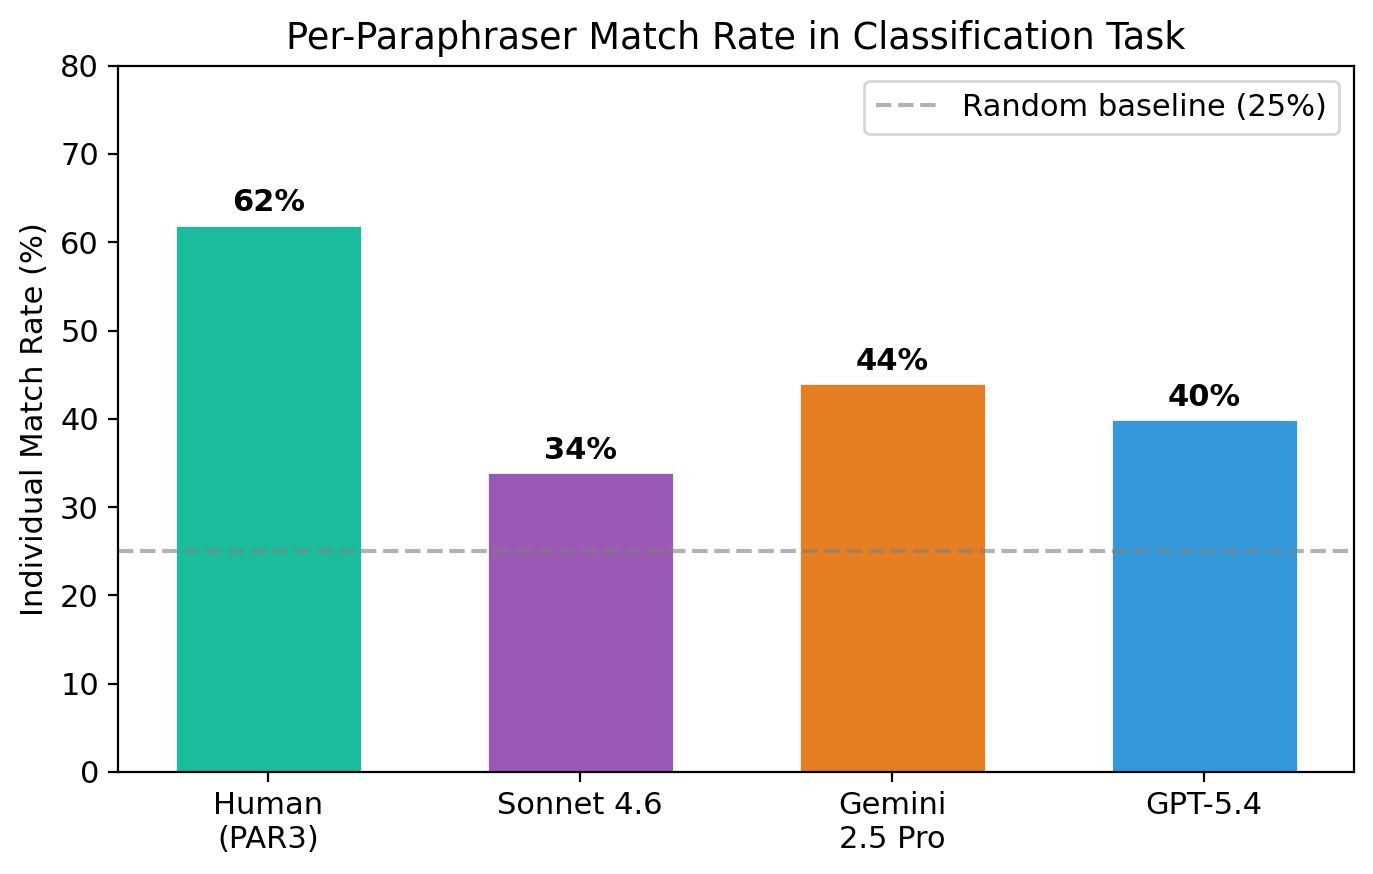
\includegraphics[width=0.85\linewidth]{figures/fig2_paraphraser_matchrate.png}
    \Description{Bar chart showing match rates: Human 62\%, Gemini 44\%, GPT-5.4 40\%, Sonnet 34\%.}
    \caption{Individual match rate per paraphraser in the classification task. Human (PAR3) translations are the easiest to identify (62\%), while Sonnet~4.6 is hardest (34\%). Random baseline is 25\%.}
    \label{fig:matchrate}
\end{figure}

Per-paraphraser match rates (Figure~\ref{fig:matchrate}) reveal a clear hierarchy:
\begin{itemize}
    \item \textbf{Human (PAR3)}: 62\%---the most identifiable. Human translators produce distinctive styles (e.g., archaic phrasing, literary flourishes) that are consistent across different source texts.
    \item \textbf{Gemini 2.5 Pro}: 44\%.
    \item \textbf{GPT-5.4}: 40\%.
    \item \textbf{Sonnet 4.6}: 34\%---closest to random (25\%), making it the best ``disguiser.''
\end{itemize}

That human paraphrases are the easiest to detect is a key finding: human rewriters exhibit more consistent personal style than LLMs, whose outputs are more variable across different inputs.

\paragraph{Confusion Analysis.}

\begin{figure}[t]
    \centering
    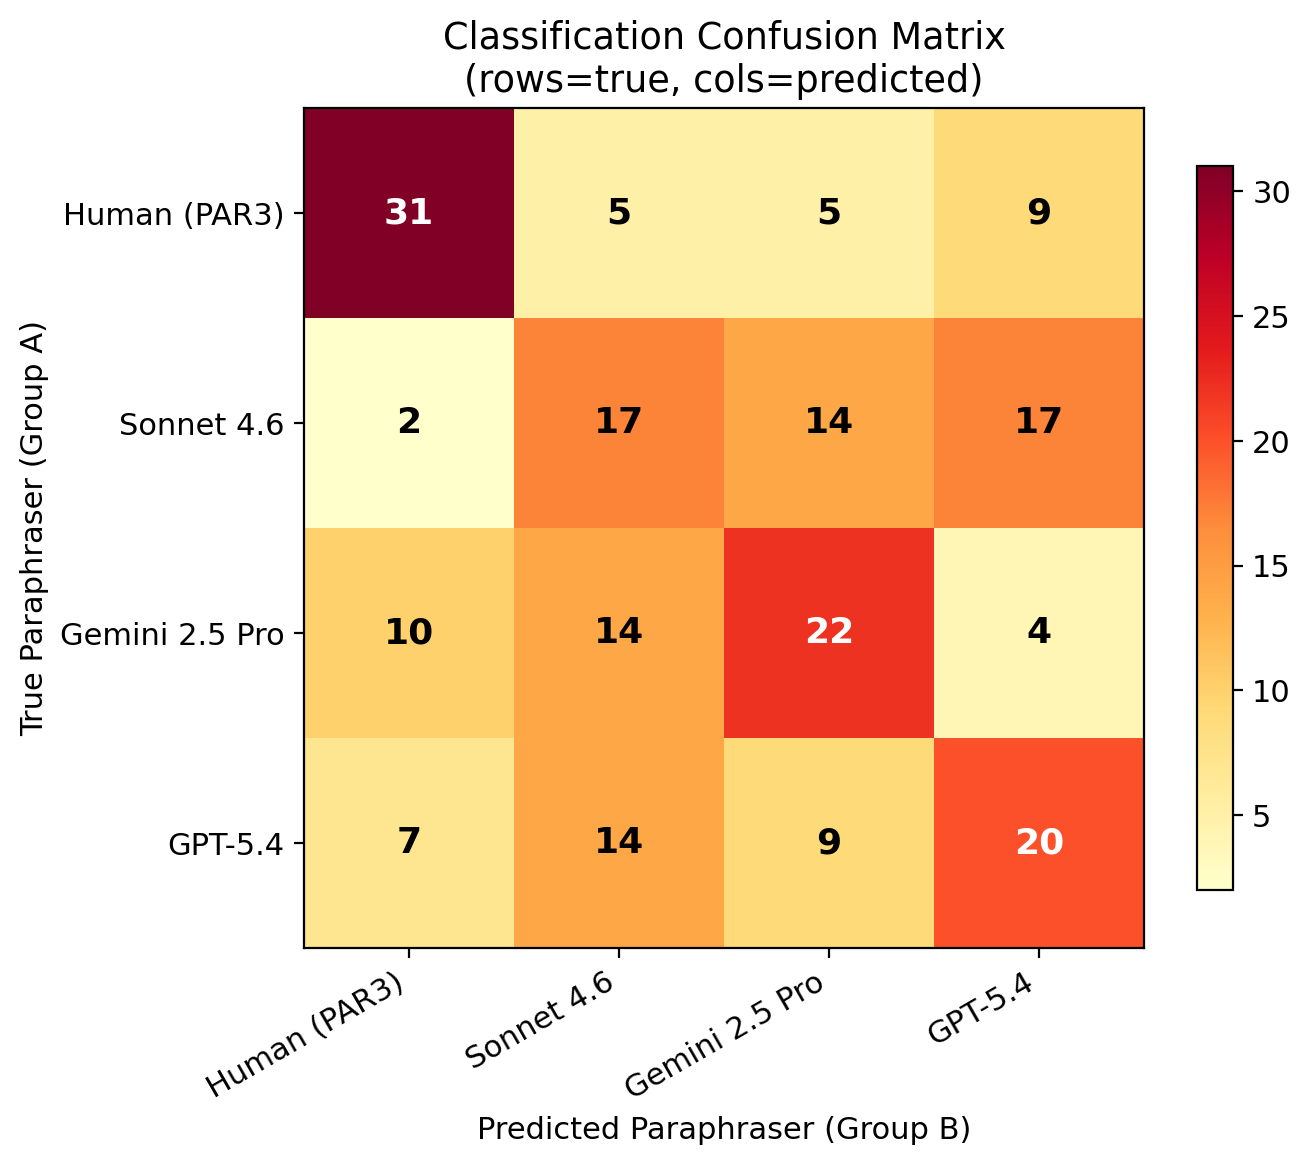
\includegraphics[width=0.85\linewidth]{figures/fig6_classification_confusion.png}
    \Description{4x4 heatmap showing classification confusion between paraphrasers.}
    \caption{Classification confusion matrix. Diagonal entries (correct matches) are strongest for Human (31) and weakest for Sonnet~4.6 (17). Off-diagonal patterns show systematic confusions between LLM paraphrasers.}
    \label{fig:confusion}
\end{figure}

The confusion matrix (Figure~\ref{fig:confusion}) reveals which paraphrasers the Detective systematically confuses.
The diagonal (correct identifications) is strongest for Human~(31/50) and weakest for Sonnet~4.6~(17/50).
Off-diagonal entries show that the three LLM paraphrasers are frequently confused with each other, while the Human is rarely mistaken for an LLM---its fingerprint occupies a distinct region of style space.

% ============================================================
\section{Summary of All Experiments}
% ============================================================

\begin{figure}[t]
    \centering
    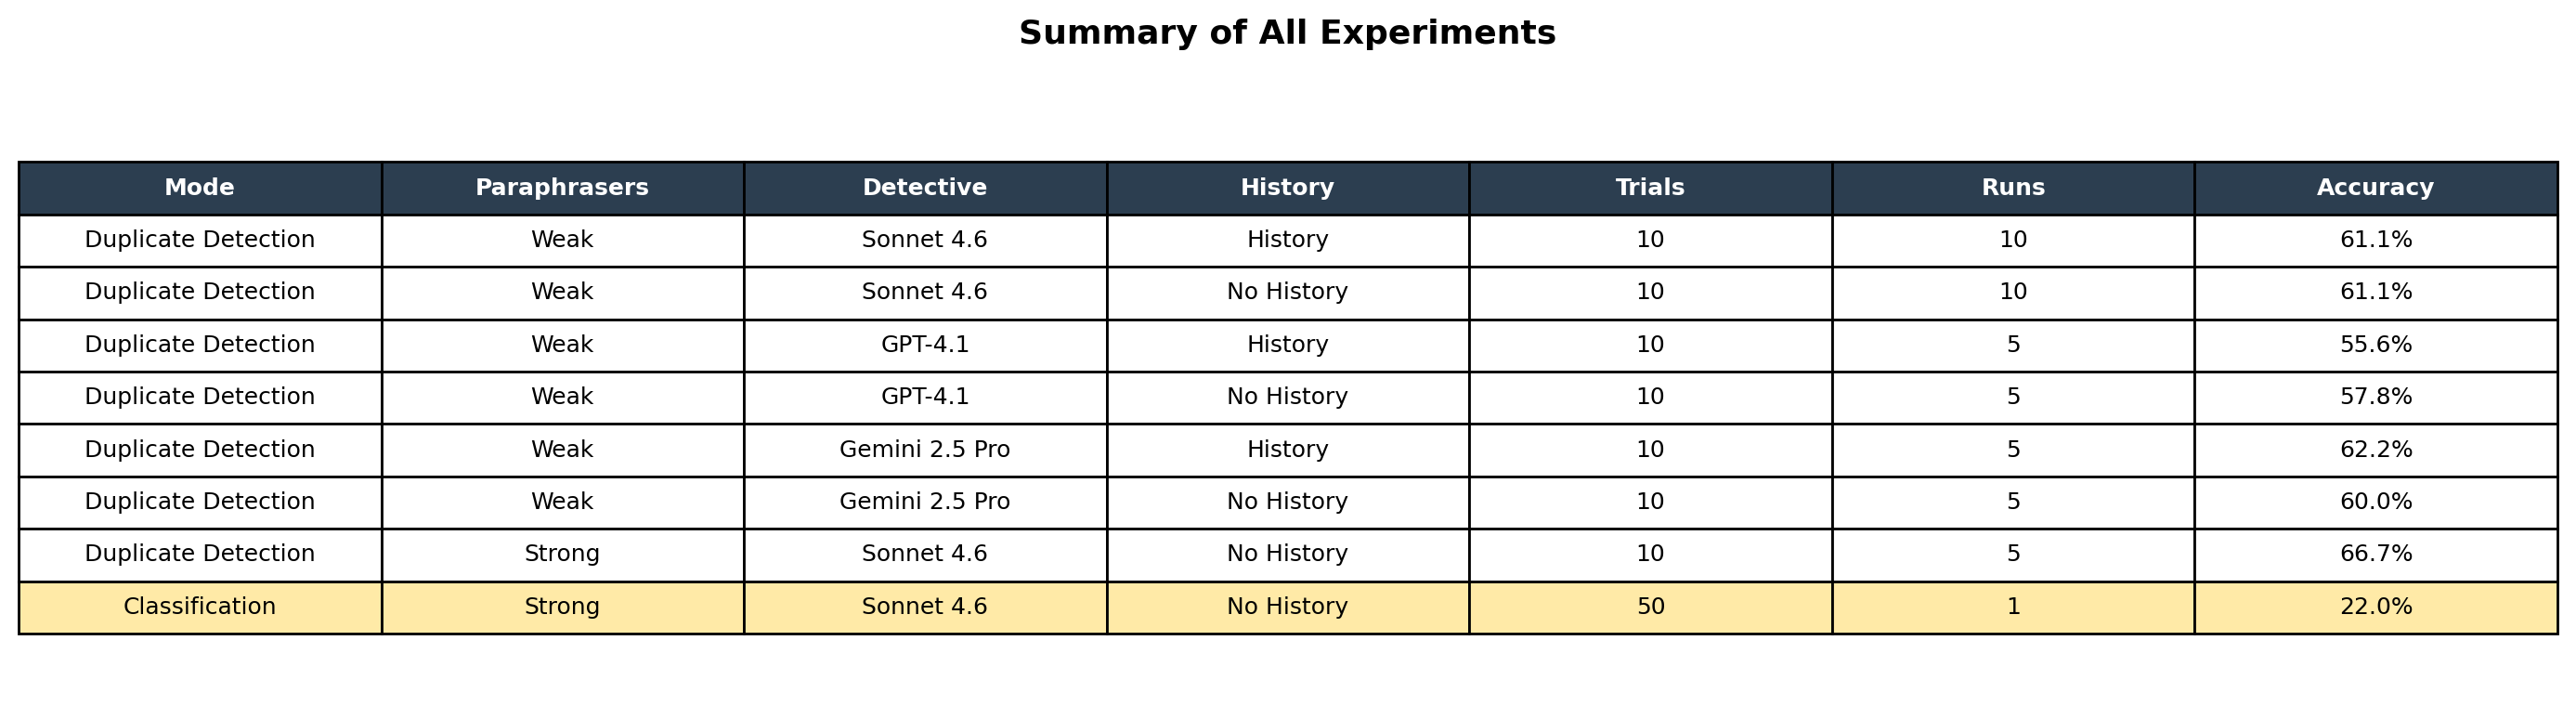
\includegraphics[width=\linewidth]{figures/fig5_summary_table.png}
    \Description{Summary table of all experimental configurations and results.}
    \caption{Summary of all experimental configurations. Eight distinct conditions were tested spanning two evaluation modes, two paraphraser strength levels, three Detective models, and two history conditions.}
    \label{fig:summary}
\end{figure}

Figure~\ref{fig:summary} presents the complete experimental matrix.
Key takeaways:
\begin{enumerate}
    \item \textbf{Fingerprints are real.} All conditions far exceed their respective random baselines (10\% for duplicate detection, 4.17\% for classification).
    \item \textbf{History does not help.} Across all Detective models, providing past trial history yields no improvement over stateless detection.
    \item \textbf{Stronger models have stronger fingerprints.} The strong paraphraser set (66.7\%) is more detectable than the weak set (61.1\%) in duplicate detection.
    \item \textbf{Humans are the most identifiable.} In the classification task, human translations from PAR3 have the highest individual match rate (62\%), consistent with the intuition that human rewriters have more distinctive personal styles.
    \item \textbf{Pairwise classification is hard but feasible.} At 22\% perfect-match accuracy (5.3$\times$ baseline), the Detective can sometimes identify all four fingerprints purely from stylistic analysis.
\end{enumerate}

% ============================================================
\section{Conclusion}
% ============================================================

We have demonstrated that different paraphrasing systems---both human and machine---leave detectable fingerprints in their outputs.
Our evaluation spans two complementary paradigms (duplicate detection and pairwise classification), three Detective models, two paraphraser strength levels, and over 400 scored trials.

The most surprising finding is that \emph{human} paraphrases are the easiest to identify, and \emph{stronger} LLM paraphrasers are more detectable than weaker ones.
This suggests that fingerprint strength correlates with the consistency of a system's ``voice''---capable models and experienced human translators develop distinctive styles that persist across different inputs.

These results open avenues for paraphraser attribution, AI text provenance, and deeper understanding of how different systems---human and machine---shape language when rewriting.

\paragraph{Code Availability.} All code and experimental data are available at \url{https://github.com/zboyr/HideNSeek}.

\bibliographystyle{ACM-Reference-Format}
\begin{thebibliography}{2}
\bibitem{mitchell2023detectgpt}
Eric Mitchell, Yoonho Lee, Alexander Khazatsky, Christopher D. Manning, and Chelsea Finn. 2023. DetectGPT: Zero-Shot Machine-Generated Text Detection using Probability Curvature. In \emph{Proceedings of ICML 2023}.

\bibitem{par3}
Eleftheria Briakou, Sweta Agrawal, Joel Tetreault, and Marine Carpuat. 2023. Searching for Relevant Translations in Parallel Corpora for Paraphrase Generation. In \emph{Findings of ACL}.
\end{thebibliography}

\end{document}
